\subsection{Navbar e sidebar}
Una volta effettuato l'accesso, l'utente si trovava davanti a una schermata principale di lavoro composta da una navbar, tramite la quale era possibile accedere alle notifiche, cambiare tema e gestire le impostazioni del profilo, e da una sidebar sulla sinistra che elencava le sezioni principali dell'applicazione: \textit{MyAcademia Dashboard}, \textit{I Miei Appunti}, \textit{Esplora Appunti}, \textit{Sbobinatore AI}, \textit{Audio Note AI} e \textit{StudyFlow AI}. Questa configurazione risultava difficile da interpretare per due motivi principali: i nomi delle sezioni non comunicavano chiaramente la loro funzionalità e alcuni erano in inglese, in contrasto con il resto dell'interfaccia in italiano. Inoltre le notifiche non erano funzionanti. Per tali ragioni si è deciso di riprogettare la navbar e la sidebar, mantenendo invariata la struttura generale e intervenendo principalmente sulla chiarezza e la coerenza linguistica dei contenuti.

\paragraph{Design pattern applicati}
\begin{itemize}
  \item \textbf{Sign-In Tools} (Tidwell): Il pattern prevede di posizionare nella parte superiore destra dell'interfaccia gli strumenti trasversali legati all'esperienza dell'utente autenticato, accessibili da qualunque schermata indipendentemente dalla sezione aperta. Alcune voci possono essere esposte direttamente come icone nella navbar, mentre altre possono essere nascoste in un menu a tendina accessibile dal nome utente o dall'avatar. Nella versione riprogettata di BrainBox, la navbar è stata arricchita rendendo funzionanti le notifiche e aggiungendo un accesso diretto al calendario, entrambi espandibili a tendina, mantenendo il nome utente con menu a tendina per le impostazioni del profilo e il logout.

    Problemi di usabilità risolti:
    \begin{itemize}
      \item P12 (Notifiche non funzionanti): Sono state attivate le notifiche, per permettere all'utente di ricevere avvisi riguardanti scadenze e attività della community.
      \item P88 (Calendario non funzionante): E' stato reso funzionante il calendario e collocato nella navbar, a differenza della versione precedente nella quale era visibile solo accedendo alla sezione \textit{Exam Details}.
    \end{itemize} 
\end{itemize}

\paragraph{Altre modifiche} 
Il testo della sidebar e della navbar è stato tradotto in italiano per garantire coerenza linguistica con il resto dell'interfaccia. Le sezioni sono state rinominate con etichette più immediate e comprensibili: \textit{Dashboard}, \textit{Appunti}, \textit{Esami} e \textit{Community}. Le due sezioni dedicate agli strumenti AI, sbobinatore e generatore di audio note, sono state accorpate all'interno di \textit{Appunti}: nella versione precedente, le trascrizioni e le audio note generate venivano salvate nelle rispettive sezioni dedicate, impedendo all'utente di organizzarle insieme agli altri file nelle cartelle di \textit{Appunti}. Centralizzando tutto in un'unica sezione, l'utente può gestire e riorganizzare liberamente l'intero materiale di studio in un solo posto. \\

Problemi di usabilità risolti:
\begin{itemize}
  \item
  \begin{itemize}
      \item P90 (”Your Exams” accessibile tramite ”StudyFlow AI”, collocata in ”Strumenti AI”, il che risulta poco pertinente rispetto alla sua funzione): La sezione per accedere ai propri esami è stata rinominata \textit{Esami} ed è stata rimossa l'etichetta \textit{Strumenti AI} perchè le funzionalità AI sono state accorpate in \textit{Appunti}.
  \end{itemize}
\end{itemize}

\begin{figure}[H]
    \centering
    
\includegraphics[width=0.8\textwidth]{figures/fig-riprogettazione-fisica/navbar-sidebar/navbar.png}
    \caption{Navbar}
    \label{fig:navbar}
\end{figure}

\begin{figure}[H]
    \centering
    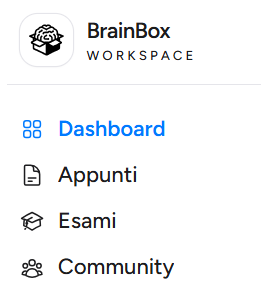
\includegraphics[width=0.3\textwidth]{figures/fig-riprogettazione-fisica/navbar-sidebar/sidebar.png}
    \caption{Sidebar}
    \label{fig:sidebar}
\end{figure}

\begin{figure}[H]
    \centering
    \begin{subfigure}[b]{0.47\textwidth}
        \centering
        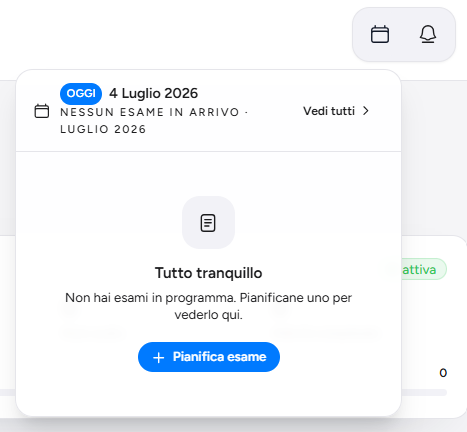
\includegraphics[width=0.8\textwidth]{figures/fig-riprogettazione-fisica/navbar-sidebar/calendario.png}
        \caption{Calendario}
        \label{fig:calendario_navbar}
    \end{subfigure}
    \qquad
    \begin{subfigure}[b]{0.47\textwidth}
        \centering
        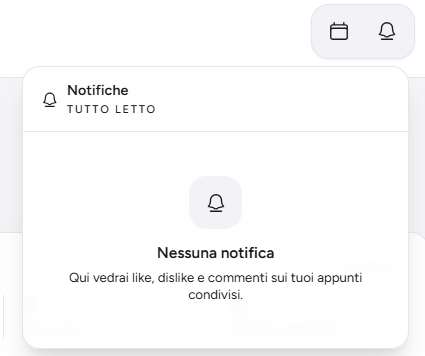
\includegraphics[width=0.8\textwidth]{figures/fig-riprogettazione-fisica/navbar-sidebar/notifiche.png}
        \caption{Notifiche}
        \label{fig:notifiche_navbar}
    \end{subfigure}

    \caption{}
    \label{fig:calendario_notifiche}
\end{figure}
